\documentclass[12pt,letterpaper]{report}
\usepackage[utf8]{inputenc}
\usepackage{amsmath}
\usepackage{amsfonts}
\usepackage{amssymb}
\usepackage{graphicx}
\usepackage[hidelinks]{hyperref}
\usepackage[T1]{fontenc}
\usepackage{lmodern}

\usepackage[authoryear,round,sort]{natbib}
\bibliographystyle{plainnat}

\title{A database for global sustainable accounting}


\begin{document}
\maketitle

Environmentally extended Multi Regional Input Output tables and analysis (EE MRIOs) have emerged as one of the main tools to analyze resource use and environmental impacts across international supply chains. They provide insights into the life cycle impacts of the production and consumption of commodities world wide, taking into account the global supply chain of purchased commodities.

Currently half a dozen EE MRIO databases are available which differ in their environmental and economic focus as well as in the level of detail. As these databases become increasingly large, it has become increasingly difficult for the non-input-output expert to access the most important attributes and results of basic calculations.

Here we present an unifying web-platform, the Environmental Footprints Explorer (http://www.environmentalfootprints.com), designed to access indicator results calculated based on these databases. The main functionality of the web-platform include (1) exploring environmental accounts based on a single database (2) comparison between databases using a common classification system and (3) exporting analysis results visualization.

The presented web-platform removes the obstacle for policy-makers and the public alike to access EE MRIO results. 


\section{Introduction}

Evidence guided policy making aiming for lessen the environmental and social
impacts of our society require a comprehensive accounting principle. 

Global Environmentally Extended Multi Regional Input-Output (EE MRIO) tables provide such an system by taking into account the interrelations between production and consumption.
Analysing EE MRIO databases require a certain degree of training and the
increasing size of the underlying matrices also set high requirements used hardware. Thus, although most of the databases are free to use the detailed results of the analysis of these databases are often hidden in the supplements of scientific articles and reports.
Here we present the Environmental Footprints Explorer (Figure \ref{fig:startpage}), http://www.environmentalfootprints.org , a web platform which provide access to the calculated results of
various EE MRIO databases. The platform also allows to compare the results across databases in a consistent classification. 

\begin{figure}[h!]
\centering
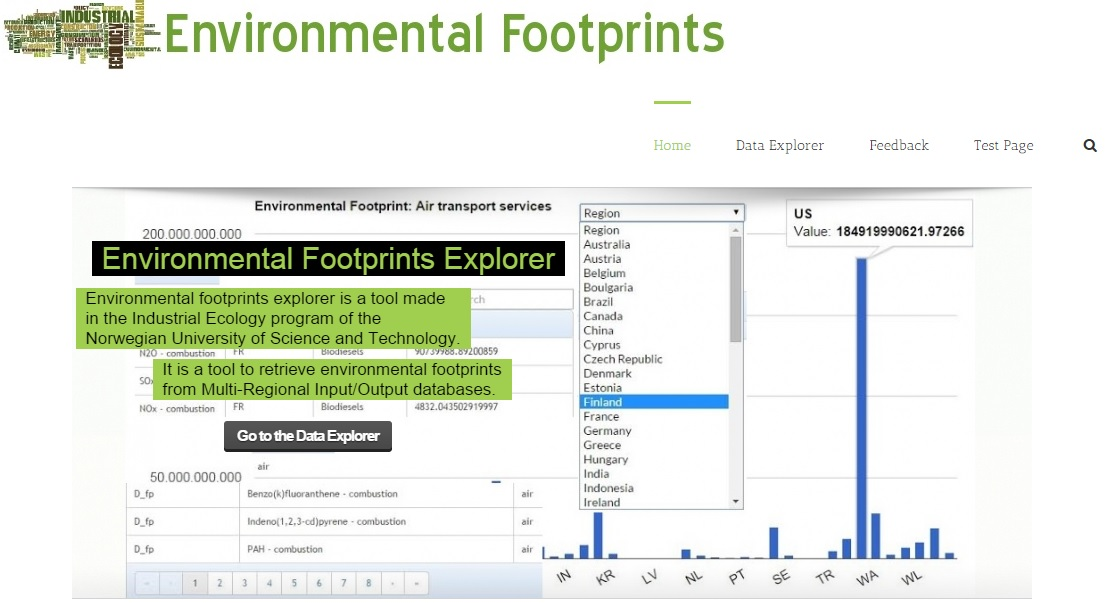
\includegraphics[width=1.0\columnwidth]{figures/web1/web1.jpg}
\label{fig:startpage} The Environmental Footprints Explorer 
\end{figure}

\label{fig:startpage} The Environmental Footprints Explorer 
%The rest of the article unfolds as follows. In the next section we give some background information on environmental accounting followed by an
overview about recently published EE MRIO databases. 
The development section describes the architecture of the
web platform and the routines used for calculating the results. We then present
the platform and highlight some use cases. We conclude with a description of
the future development.
%\subsection{Environmental Accounting}

%Principally, pressures arising from economic activity can either be tallied at
the actual place of production or at the point of the consumption.
Traditionally, the accounting at the actual place of production has been used
for policy decisions. For example, the Kyoto Protocol was based on the
production principle, which is now discussed to be one of the reasons for its
limited success \cite{23192129}. 

Consumption based accounting (CBA), on the other hand, just recently gained
momentum for policy making \cite{Harris_2013}. In CBA, all resource use and environmental
pressurs (for example emissions) occurring along the the supply chain of
products are added up and allocated to the final consumer of the product. This
allows for example to assess the environmental pressure caused by a domestic
demand abroad \cite{Weinzettel_2013, 20212122}.

Indicators based on consumption based accounting are also known as various
types of 'footprints' and are increasingly used for informing policy makers as
well as the public about ongoing environmental \cite{tukker_global_2014, steen-olsen_carbon_2012, Kanemoto_2014, united_nations_university_inclusive_2012}
and social problems \cite{Simas_2014}. 

CBA requires a comprehensive description of the global socio-economic
metabolism including among other the structure of domestic economies, their
ressource use and the amount of trade between countries and regions.
Environmentally Extended Multi Regional Input-Output databases (EEMRIO) provide
all these data in a consistent framework. 
%\subsection{EE MRIO database}


%\subsubsection{EXIOBASE}


EXIOBASE is a global EE MRIO aiming to support analysis of technologies,
policies, and standards in relation to EU sustainability policies. The
environmental focus of the database reflect in a high level of detail in the
agriculture, energy, mining, trans- port, and waste management sectors. In
addition, EXIOBASE provides satellite accounts for over 300 environmental
interventions.  

The database was developed and analysed in three consecutive EU projects: EXIOPOL \cite{Tukker_2013}, CREEA \cite{Wood_2014} and the ongoing project DESIRE. The currently available version, EXIOBASE 2, implements the
economic and environmental accounting principles proposed in the UN System of
Economic and Environmental Accounts \cite{european_commission._system_2014}.
The ongoing development of EXIOBASE 3 concentrates on providing a time series
of EE MRIOs and now-casting this time series to the current year. 

Currently, EXIOBASE consists of EE MRIOs for 26 (27 in the upcoming version 3) EU countries
and 16 major economies in industry and industry (163 sectors) as well as
product by product (200 sectors) classification.
%asdf
%\subsubsection{2.2.3 Eora}


Eora is a time-series (1990-2009 of input-output tables with high country detail (150 or so), utilising assymetric levels of detail and concepts of supply-use. There is further a smaller version of Eora at 26 sectors common for all countries.
%\section{Database description}

%Calculation of EE MRIO accounts (Multipliers, Footprints, ...) followed
standard IO methodology. We used the open source tool pymrio (https://github.com/konstantinstadler/pymrio) for the calculations.

Data aggregated to a common classification as described in Kjartan..
%In order to compare the different EE MRIOs included, we aggregated each into the Common Classification System \cite{Steen_Olsen_2014}. 
This system comprises the common denominator for all EE MRIOs available and leads to an aggregation to 41 regions (40 countries and 1 Rest of the World, \ref{tab:cc_sectors}) and 17 sectors (\ref{tab:cc_regions}). 
Due to the European focus of most EE MRIO projects, the Common Classification includes all European Union countries (except the new member state Croatia).


\begin{table}
\label {tab:cc_regions}
\begin{tabular}{ c c c l }
\textbf{Number} & \textbf{ISO3 Code} & \textbf{UN Code} & \textbf{Name}\\
1&AUS & 36 & Australia\\
2&AUT & 40 & Austria\\
3&BEL & 56 & Belgium\\
4&BRA & 76 & Brazil\\
5&BGR & 100 & Bulgaria\\
6&CAN & 124 & Canada\\
7&CHN & 156 & China\\
8&CYP & 196 & Cyprus\\
9&CZE & 203 & Czech Republic\\
10&DNK & 208 & Denmark\\
11&EST & 233 & Estonia\\
12&FIN & 246 & Finland\\
13&FRA & 250 & France\\
14&DEU & 276 & Germany\\
15&GRC & 300 & Greece\\
16&HUN & 348 & Hungary\\
17&IND & 356 & India\\
18&IDN & 360 & Indonesia\\
19&IRL & 372 & Ireland\\
20&ITA & 380 & Italy\\
21&JPN & 392 & Japan\\
22&LVA & 428 & Latvia\\
23&LTU & 440 & Lithuania\\
24&LUX & 442 & Luxembourg\\
25&MLT & 470 & Malta\\
26&MEX & 484 & Mexico\\
27&NLD & 528 & Netherlands\\
28&POL & 616 & Poland\\
29&PRT & 620 & Portugal\\
30&ROM & 642 & Romania\\
31&RUS & 643 & Russia\\
32&SVK & 703 & Slovakia\\
33&SVN & 705 & Slovenia\\
34&KOR & 410 & SouthKorea\\
35&ESP & 724 & Spain\\
36&SWE & 752 & Sweden\\
37&TWN & n.a. & Taiwan\\
38&TUR & 792 & Turkey\\
39&GBR & 826 & United Kingdom\\
40&USA & 840 & United States\\
41& RoW & n.a. & Rest of the World\\
\end{tabular}
\caption{Countries and regions of the MRIOs included in the Environmental Footprint Explorer. 
The original countries of the MRIOs were modified to have a comparable country set for each MRIO. The new set includes the EU countrie except Croatia (EU27) and other major economies accounting for about 90 of the global GDP \cite{Stadler_2014}. UN codes for Taiwan and the aggregated RoW are not available (n.a.).}
\end{table}


\begin{table}
\label {tab:cc_sectors}

\begin{tabular}{ c c l }
\textbf{Number} & \textbf{Code} & \textbf{Name }\\
1 &  AGRF &  Agriculture, forestry, hunting, and fisheries\\
2 &  MINQ &  Mining and quarrying\\
3 &  FOOD &  Food products, beverages, and tobacco\\
4 &  CLTH &  Textiles, leather, and wearing apparel\\
5 &  WOOD &  Wood, paper, and publishing\\
6 &  PETC &  Petroleum, chemical, and non-metal mineral products\\
7 &  METP &  Metal and metal products\\
8 &  ELMA &  Electrical equipment and machinery\\
9 &  TREQ &  Transport equipment\\
10 &  MANF &  Manufacturing and recycling\\
11 &  ELGW &  Electricity, gas and water\\
12 &  CNST &  Construction\\
13 &  TRAD &  Trade\\
14 &  TRNS &  Transport\\
15 &  POST &  Post and telecommunications\\
16 &  BSNS &  Financial intermediation and business activities\\
17 &  PAEH &  Public administration, education, health, recreational, and other services\\
\end{tabular}

\caption{Sectors of the MRIOs included in the Environmental Footprint Explorer. The original classification of the MRIOs were aggregated into the Common Classification System \cite{Steen_Olsen_2014} in order to make them comparable.}
\end{table}



%For the data storage the MySQL RDBMS was used.
The results of the calculation which were in csv format files was used to update mysql database table on web server. Wordpress CMS was used for web development. The tool for data exploration was done using wordpress plugin which query data, using php, directly from mysql database table. The data are shown in html table with possibility to select and filter different options. Visualization of data was interpreted using plotly web tool based on d3js.  


%\section{Tool description}

The interactive database provides three main functions. In the following three sections we describe each function and give a short example of a possible use case.
%\subsection{Viewing EE MRIO accounts based on a specific database}

Users can specify one of the freely available EE MRIO databases. 
Within a database, several parameters can be selected (Figure \ref{fig:select}). These include:

\begin{itemize}
    \item Countries/regions available in the selected database
    \item Sector of the database
    \item Environmental/social intervention
    \item Year
    \item Perspective (Footprint, production/territorial accounts, embodied
      pressures/impacts in imports and exports, Multipliers and Intensities)
\end{itemize}


The general idea behind the selection is that the user specifies four out
of five parameters and gets an overview of remaining parameter.

For example, choosing the database EXIOBASE for 2007 and specifying export accounts for the perspective, CO_2 as the environmental intervention, and air transport service as sector result in a result list showing these paramters accros regions (the undefined parameter, see Figure \ref{fig:table}).

%\begin{figure}[h!]
%\centering
%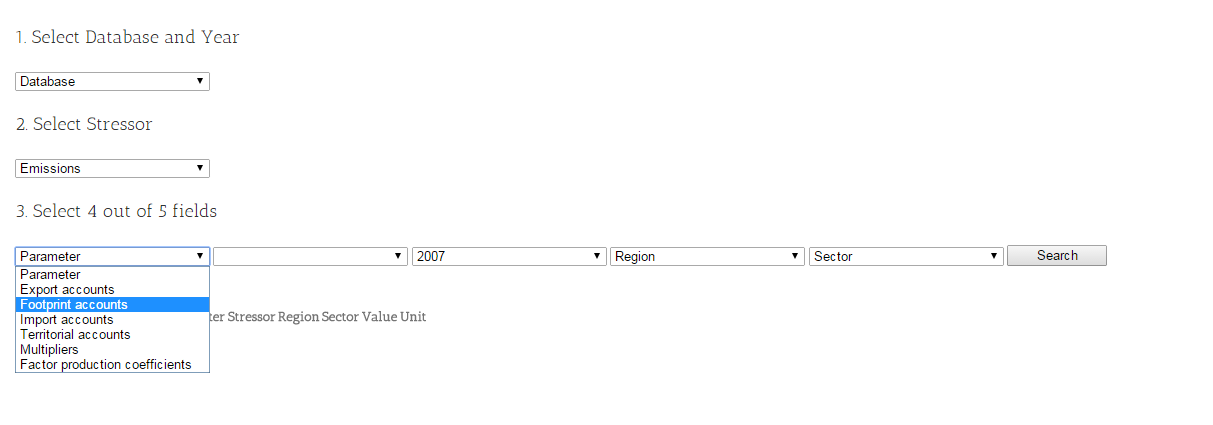
\includegraphics[width=1.0\columnwidth]{figures/mrioweb/mrioweb.png}
%Fig. 2 The Environmental Footprint Explorer aim to ease the data extraction from global EE MRIO databases. Users can select between different databases and specify the perspectives, region and sectors they are interested in.
%\end{figure}

%\subsection{Comparing accounts across databases in a common classification system}

The main problem in any EE MRIO comparison is the sector and accounting
mismatch between the databases. To solve that issue, we aggregated every
database into a Common Classification System \cite{Steen_Olsen_2014}. 

Leaving the model field in the selection unspecified allows to compare results across databases. 
In addition, we compiled one additional database based on the average results of all included MRIOs.


%The Environmental Footprints Explorer provides a consistent way to access environmental accounts of different EE MRIO databases and also to compare these results across databases.

The implementation of the Environmental Footprints Explorer allows to easily extend the number of EE MRIO databases accessible. In the short term, all EXIOBASE versions, WIOD and the aggregated EORA system will be integrated. 
%Some recent studies analyzed the differences between EE MRIO databases \cite{Stadler_2014, Owen_2014, Moran_2014}. This studies provided important background information on the reasons for the observed differences and some exemplified comparison on the effect of the differences on indicators. In order to get the amount of difference for other indicators, any practitioner would need to redo the whole study, starting from parsing several EE MRIO databases, aggregating to a common system and re-analyze the indicator results. 

The proposed web-platform provides a different approach. The comparison of the EE MRIO databases is readily available through the user interface as is the access to the detailed results.
%In the next couple of month, we plan to extend the number of EE MRIO included in the comparison. The upcoming update of EXIOBASE to version 3 (February 2016) will be included in the web-platform providing the first now-casted EE MRIO results. In addition, we will contact other EE - MRIO database providers to discuss a potential inclusion of their data into the unified web-platform.
%\subsection{Downloading results and API}

The data extracted in the two use cases described above gets presented in a table together with a visualization. Both items can be downloaded (as csv file and png graphics).

In addition, the web-interface also provides an API access to the databases. 

\textbf{Draft Note: This will be implemented in May and will be available at the time of the presentation. We plan to include a supplement describing the API commands to access the database and to exemplify  an use case here.}



%\begin{figure}[h!]
%\centering
%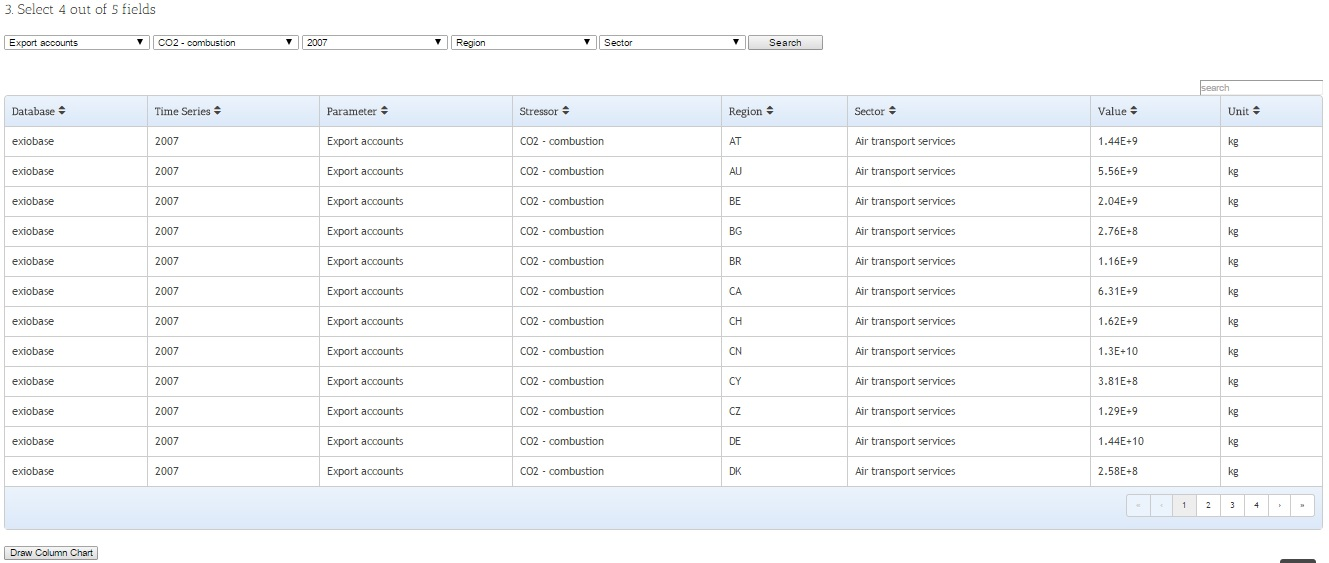
\includegraphics[width=1.0\columnwidth]{figures/web6/web6.jpg}
%\label{fig:table} Results of a data query are presented as a table.
%\end{figure}


%\begin{figure}[h!]
%\centering
%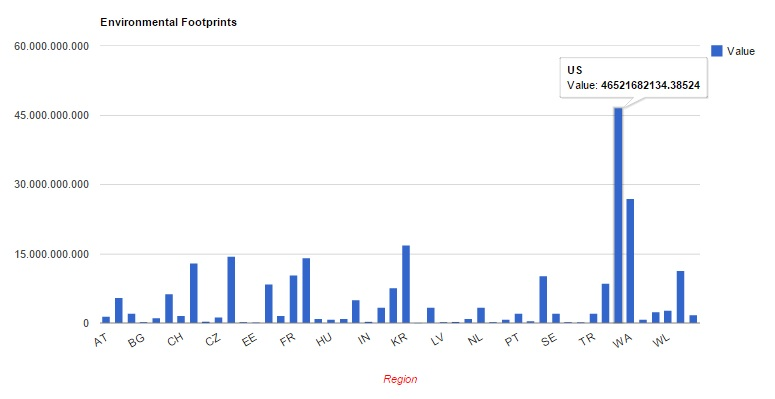
\includegraphics[width=1.0\columnwidth]{figures/web7/web7.jpg}
%\label{fig:bar} An automatic visualization procedure provides a quick overview about the extracted data.
%\end{figure}

%\section{Conclusion and outlook}

Here we described an integrated web-interface, the Environmental Footprints Explorer, developed to ease the access to EE MRIO results. The platform provides functionality for the in depth exploration of a single database as well as for the comparison across several EE MRIO databases.

Although several EE MRIO have been developed and published in the past couple of years, the use of their results in informing the policy development process has been potentially limited. The reasons for that, are on the one hand, some expertise are needed to calculate indicators based on EE MRIO accounting, and on the other hand due to the often overwhelming amount of data provided by current EE MRIO databases.

Some EE MRIO projects have tried to overcome that problem in the past by providing various kind of open access result reporting. For example, the OPEN:EU projects provides the policy tool EUREAPA to allow easy access to environmental and economic data for an EE MRIO model based on GTAP \cite{Roelich_2014}. The EE MRIO Eora \cite{Lenzen_2013} includes a web-interface to access the main results (http://worldmrio.com) and the EXIOBASE project provide a booklet summarizing the main results for a policy audience \cite{tukker_global_2014}. Similar initiatives exist also on the national level, for example the Open IO-Canada allows to retrieve environmental information based on the Canadian economic input-output tables (http://ciraigdev.polymtl.ca). However, all these initiatives fall short in enabling a comparison across databases.  

The overall goal of the Environmental Footprints Explorer is to deliver the newest environmental accounting results to policy makers and the public. Previously, these data was filtered by the analyst of the databases and often restricted to the top level results considered novel enough for a scientific publication. Detailed data or the newest updates of previously published data may still be hidden in the databases, although they could be critical for informing targeting policy development.

Recently, the European Science Policy (http://ec.europa.eu/programmes/horizon2020/en/h2020-section/open-science-open-access) as well as various scientific journals \cite{Hanson_2011, Stodden_2012, Boulton_2012} committed to a open science and data scheme. We feel, that, in an ideal situation, open science should not only provide open access to the raw data used for any analysis, but also provide a way to utilize the data for non-experts. The Environmental Footprints Explorer represents a first step in that direction.
    
    
    
%Here we described an unifying web-interface developed in order to simplify the access to EE MRIO results. The platform provides functionality for the in depth exploration of a single database as well as for the comparison across several EE MRIO databases.
%Although several EE MRIO have been developed and published in the past couple of years, the use of their results in informing the policy development process has been rather limited. 

The reason for that being are that on one hand that some expertise are needed to calculate indicators based on EE MRIO accounting, on the other hand the often overwhelming amount of data provided by current EE MRIO databases.

Some EE MRIO projects have tried to overcome that problem in the past by providing various kind of open access result reporting. For example, the OPEN:EU projects provides the policy tool EUREAPA to allow easy access to environmental and economic data for an EE MRIO model based on GTAP \cite{Roelich_2014}. The EE MRIO Eora \cite{Lenzen_2013} includes a web-interface to access the main results (http://worldmrio.com) and the EXIOBASE project provide a booklet summarizing the main results for a policy audience \cite{tukker_global_2014}. Similar initiatives exist also on the national level, for example the Open IO-Canada allows to retrieve environmental information based on the Canadian economic input-output tables (http://ciraigdev.polymtl.ca).


%The overall goal of the Environmental Footprints Explorer is to deliver the newest environmental accounting results to policy makers and the public. Previously, these data was filtered by the analyst of the databases and often restricted to the top level results considered novel enough for a scientific publication. Detailed data or the newest updates of previously published data may still be hidden in the databases, although they could be critical for informing targeting policy development.

Recently, the European Science Policy (http://ec.europa.eu/programmes/horizon2020/en/h2020-section/open-science-open-access) as well as various scientific journals (\cite{Hanson_2011} \cite{Stodden_2012}, \cite{Boulton_2012}) committed to a open science and data scheme. 

\bibliography{bibliography/biblio}
\end{document}
